% -*- latex -*-

\chapter{Customizing Compositing}
\label{chap:Customizing_Compositing}

If you have been reading this document from the beginning, then you already
know enough to use \IceT for many typical rendering applications.  Chapters
\ref{chap:Tutorial} and \ref{chap:Basic_Usage} describe how to build and
link \IceT, establish an \IceT context in your application, and to leverage
\IceT to make your rendering parallel.  This chapter describes the many
features \IceT provides to let you customize the image compositing to your
application.

\section{Compositing Operation}
\label{sec:Customizing_Compositing:Compositing_Operation}
\index{compositing|(}
\index{compositing~operation|(}

\IceT is classified as a \index{sort-last}\keyterm{sort-last} type of
parallel rendering library, as discussed in
Chapter~\ref{sec:Introduction:Parallel_Rendering_Primer}.  Basically, this
means that each process renders images independently, and then these
images, each comprising a different partition of the geometry, are combined
together in a process called \keyterm{compositing}.

To combine two images together, a \keyterm{compositing operation} is
applied to every corresponding pair of pixels.  Three or more images are
combined by applying the compositing operation multiple times to eventually
reduce everything to one image.  (The compositing operations supported by
\IceT are associative, so the order is flexible.  \IceT takes advantage of
this fact to efficiently perform the compositing in parallel.)

\IceT supports two compositing operations, set with
\CFunc{icetCompositeMode}.

\begin{Table}{3}
  \textC{void }\CFunc{icetCompositeMode}\textC{(}&\textC{IceTEnum}&\CArg{mode}\quad\textC{);}
\end{Table}

The first type of compositing operation,
\CEnum{ICET\_COMPOSITE\_MODE\_Z\_BUFFER}, is a depth comparison and the
other, \CEnum{ICET\_COMPOSITE\_MODE\_BLEND}, is an alpha blend.  The depth
comparison is a bit faster and is easier to use, but only works for opaque
surfaces.  If you are performing \index{volume~rendering}\keyterm{volume
  rendering}, the translucent rendering of 3-dimensional volumes, or any
other rendering that involves transparent data, then you will have to use
the alpha blend compositing operation.

Each compositing operation relies on certain buffers to exist (or not
exist) in images.  For example, z-buffer compositing can use a color buffer
and requires a depth buffer whereas blended compositing requires a color
buffer and cannot work with a depth buffer.  The buffers created in images
by \IceT, and their formats, is controlled by the
\CFunc{icetSetColorFormat} and \CFunc{icetSetDepthFormat} functions.  It is
important to ensure that the setting for \CFunc{icetCompositeMode} is
compatible with the settings for \CFunc{icetSetColorFormat} and
\CFunc{icetSetDepthFormat}.

\begin{Table}{3}
  \textC{void }\icetSetColorFormat\textC{(}&\textC{IceTEnum}&\CArg{color\_format}\quad\textC{);} \\
  \textC{void }\icetSetDepthFormat\textC{(}&\textC{IceTEnum}&\CArg{depth\_format}\quad\textC{);}
\end{Table}

The following \CArg{color\_format}s are valid for use in
\CFunc{icetSetColorFormat}.

% -*- latex -*-

  \begin{Description}[ICET\_IMAGE\_COLOR\_RGBA\_UBYTE]
  \item[\CEnum{ICET\_IMAGE\_COLOR\_RGBA\_UBYTE}] Each entry is an RGBA
    color tuple.  Each component is valued in the range from $0$ to $255$
    and is stored as an 8-bit integer.  The buffer will always be allocated
    on memory boundaries such that each color value can be treated as a
    single 32-bit integer.
  \item[\CEnum{ICET\_IMAGE\_COLOR\_RGBA\_FLOAT}] Each entry is an RGBA
    color tuple.  Each component is in the range from $0.0$ to $1.0$ and is
    stored as a 32-bit float.
  \item[\CEnum{ICET\_IMAGE\_COLOR\_RGB\_FLOAT}] Each entry is an RGB color
    triple. Each component is in the range from $0.0$ to $1.0$ and is
    stored as a 32-bit float. Note that there is no alpha channel, so the
    color blending composite mode will not work with this color format.
  \item[\CEnum{ICET\_IMAGE\_COLOR\_NONE}] No color values are stored in the
    image.
  \end{Description}



The following \CArg{depth\_format}s are valid for use in
\CFunc{icetSetDepthFormat}.

% -*- latex -*-

  \begin{Description}[ICET\_IMAGE\_COLOR\_RGBA\_UBYTE]
  \item[\CEnum{ICET\_IMAGE\_DEPTH\_FLOAT}] Each entry is in the range from
    $0.0$ (near plane) to $1.0$ (far plane) and is stored as a 32-bit
    float.
  \item[\CEnum{ICET\_IMAGE\_DEPTH\_NONE}] No depth values are stored in the
    image.
  \end{Description}


\subsection{Z-Buffer Compositing}
\label{sec:Customizing_Compositing:User_Defined_Communicators}
\index{z-buffer}
\index{z-buffer|seealso{compositing, z-buffer}}
\index{depth~buffer|see{compositing, z-buffer}}
\index{compositing!z-buffer|(}

\keyterm{Z-buffer compositing} takes advantage of the same hidden surface
removal already taking place in the OpenGL pipeline.  \IceT pulls the
\index{z-buffer}z-buffer (also often known as the \keyterm{depth buffer})
from the OpenGL image buffers.  The compositing operation then just
compares the depth values of two pixels and chooses the one that is closer.

Z-buffer compositing is used when the composite mode (set with
\CFunc{icetCompositeMode}) is \CEnum{ICET\_COMPOSITE\_MODE\_Z\_BUFFER}.
Z-buffer compositing also requires a depth buffer.  An error will occur
during compositing if z-buffer compositing is being used without a depth
buffer (i.e. \CFunc{icetSetDepthFormat} is set to
\CEnum{ICET\_IMAGE\_DEPTH\_NONE}.)

By default, z-buffer compositing is enabled and both the the color and the
depth buffer are selected as input buffers.  Also by default \IceT will
\emph{not} produce a depth buffer.  (Not computing the depth buffer may
save some network transfer time.)  This behavior is controlled by the
\CEnum{ICET\_COMPOSITE\_ONE\_BUFFER} option, which is enabled by default.

If you need the depth buffer composited in addition to the color buffer
(for example, to help with a picking operation), you can do so by simply
disabling the \CEnum{ICET\_COMPOSITE\_ONE\_BUFFER} option.

\begin{code}
icetCompositeMode(ICET_COMPOSITE_MODE_Z_BUFFER);
icetSetColorFormat(ICET_IMAGE_COLOR_RGBA_UBYTE);
icetSetDepthFormat(ICET_IMAGE_DEPTH_FLOAT);
icetDisable(ICET_COMPOSITE_ONE_BUFFER);
\end{code}

Alternatively, if you only need the depth buffer (for example, as a shadow
map), you can do so by setting the color format to
\CEnum{ICET\_IMAGE\_COLOR\_NONE}.  In this case, the
\CEnum{ICET\_COMPOSITE\_ONE\_BUFFER} option will have no effect

\begin{code}
icetCompositeMode(ICET_COMPOSITE_MODE_Z_BUFFER);
icetSetColorFormat(ICET_IMAGE_COLOR_NONE);
icetSetDepthFormat(ICET_IMAGE_DEPTH_FLOAT);
\end{code}

\index{compositing!z-buffer|)}

\subsection{Volume Rendering (and Other Transparent Objects)}
\label{sec:Customizing_Compositing:Volume_Rendering}
\index{blending|see{compositing, blended}}
\index{compositing!blended|(}
\index{volume~rendering|(}

A well known limitation to z-buffer compositing --- and the z-buffer hidden
surface removal algorithm in general --- is that it only works with opaque
objects.  You will get invalid results if you try to apply z-buffer
compositing on transparent objects.

There are two fundamental problems with the z-buffer compositing operation
when dealing with translucent pixels.  The first problem is that you cannot
simply pick the nearest color value.  You must \keyterm{blend} the front
pixel's color with the back pixel's color.  The second problem is that the
color blending is order dependent.  That is, you have to know which pixels
are in front of others.  Although it is technically possible to use
z-buffer values to determine the ordering of a pair of pixels, making sure
that all the pixels get composited in the correct order requires additional
information about and constraints on the geometry.

When z-buffer compositing is not applicable, you must use \keyterm{blended
  compositing}.  To use blended compositing, set the composite mode (with
\CFunc{icetCompositeMode}) to \CEnum{ICET\_COMPOSITE\_MODE\_BLEND} and turn
off depth buffers (i.e. \CFunc{icetSetDepthFormat} is set to
\CEnum{ICET\_IMAGE\_DEPTH\_NONE}).

\begin{code}
icetCompositeMode(ICET_COMPOSITE_MODE_BLEND);
icetSetColorFormat(ICET_IMAGE_COLOR_RGBA_UBYTE);
icetSetDepthFormat(ICET_IMAGE_DEPTH_NONE);
\end{code}

The blending composite operator relies on the \index{alpha}\keyterm{alpha}
(\index{$\alpha$}\keyterm{$\alpha$}) channel of the color buffer (the A in
RGBA colors).  Note that when using \OpenGL, the alpha values must actually
be available in the \OpenGL color buffers in order for blended compositing
to work.  Many applications create \OpenGL buffers without alpha bit planes
in them because they are often not necessary to render images in serial.
Make sure your application creates alpha bit planes before attempting to
composite translucent images with \IceT (or any other library).

The blending operation is the standard
\index{over~operator}\index{under~operator}\keyterm{over/under operator}
defined in the seminal 1984 Porter and Duff paper.
\begin{equation}
  C_o \leftarrow C_f + C_b (1 - \alpha_f)
  \label{eq:VolumeRendering:OverOperator}
\end{equation}
where $C$ is an RGBA color vector, $\alpha$ is the alpha component of a
color vector, and the $f$, $b$, and $o$ subscripts denote the front, back,
and output values, respectively.

Each color in Equation~\ref{eq:VolumeRendering:OverOperator} represents a
\index{pre-multiplied~color}\keyterm{pre-multiplied color}, meaning that
the red, green, and blue values are scaled by the alpha parameter.  Thus, a
fully red color at half transparency is represented by the vector $\langle
0.5, 0, 0, 0.5 \rangle$ rather than $\langle 1, 0, 0, 0.5 \rangle$.  In
pre-multiplied colors, none of the red, green, or blue values ever exceed
the alpha value.  Note that colors are often provided in \OpenGL as
non-pre-multiplied values, and the blending equation $C_o \leftarrow C_f
\alpha_f + C_b (1 - \alpha_f)$ is used instead of the one in
Equation~\ref{eq:VolumeRendering:OverOperator}.  Although this blending
gives the correct RGB color, it computes an invalid alpha parameter, so
watch out!

\index{ordered compositing|see{compositing, ordered}}
\index{compositing!ordered|(}

Simply turning on blended compositing is not sufficient to render
translucent objects.  You must also tell \IceT to perform \keyterm{ordered
  compositing}.  In ordered compositing, you must have a
\index{visibility~ordering}\keyterm{visibility ordering}.  Given any two
processes, a visibility ordering ensures and determines that all of the
geometry in one process is in front of or behind all the geometry in each
of the other process with respect to the camera.  In some cases, such as
when volume rendering a 3D Cartesian grid of points distributed in blocks
to processes, finding the visibility ordering is straightforward.  In other
cases, such as when rendering unstructured collections of polygons or
polyhedra, it can be difficult to ensure that a visibility ordering exists
and can be found.  Doing so may be the most challenging part of creating a
parallel rendering application.  An example of creating a visibility
ordering from unstructured data can be found in the ParaView application,
and the implementation is detailed in the following paper:

\begin{quote}
  Kenneth Moreland, Lisa Avila, and Lee Ann Fisk. ``Parallel Unstructured
  Volume Rendering in ParaView,'' In \emph{Visualization and Data Analysis
    2007, Proceedings of SPIE-IS\&T Electronic Imaging}, January 2007,
  pp. 64950F-1--12.
\end{quote}

Ordered compositing is turned on by simply passing the
\CEnum{ICET\_ORDERED\_COMPOSITE} flag to \CFunc{icetEnable}.
\begin{code}
icetEnable(ICET_ORDERED_COMPOSITE);
\end{code}

Once ordered compositing is enabled, it is very important to use
\CFunc{icetCompositeOrder} to specify the visibility order of the geometry
associated with each process.  This must generally be done before each call
to \CFunc{icetDrawFrame} or \CFunc{icetGLDrawFrame}.
\begin{Table}{1}
  \textC{void }\CFunc{icetCompositeOrder}\textC{(} \textC{const IceTInt *}
  \CArg{process\_ranks} \textC{);}
\end{Table}
The \CFunc{icetCompositeOrder} function takes an array of processes.  It is
assumed that the geometry of the first process in the list is in front of
the rest of the processes; the geometry of the second process in the list
is in front of all the processes except the first, and so on.  The
visibility order often changes when the camera angle changes, so it is
important to recompute and report a new composite order on every frame.

Be aware that not all strategies support ordered compositing.  If the
current strategy does not support ordered compositing, then the
\CEnum{ICET\_ORDERED\_COMPOSITE} flag is ignored.  Consult the
documentation in Chapter~\ref{chap:Strategies} or the documentation for the
\CFunc{icetStrategy} command to determine which strategies support ordered
compositing.  In any case, you can check the
\CEnum{ICET\_STRATEGY\_SUPPORTS\_ORDERING} state variable to determine if
the current compositing strategy supports ordered compositing.

\index{compositing!ordered|)}

\index{clear~color|see{background color}}
\index{background~color|(}

One final thing to worry about when using blended compositing is to make
sure that the background color does not interfere with the compositing.
Because the visibility order is important, you need to make sure that none
of the processes render with a background (except perhaps the process
nearest the rear).  For example, let us say you want to render an image
with a blue background.  Let us also say that process $A$'s geometry is in
front of process $B$'s geometry.  Process $A$ cannot render its geometry on
top of a blue background because that background should really also be
behind the geometry of process $B$, and the resulting image will be
invalid.

If your background is a solid color, then \IceT can fix this problem
automatically.  Both \CFunc{icetDrawFrame} and \CFunc{icetGLDrawFrame} have
the ability take a solid background color and modify it as appropriate for
compositing.  \CFunc{icetDrawFrame} takes the background color as an
explicit parameter whereas \CFunc{icetGLDrawFrame} implicitly gets the
background color from the \OpenGL clear color.

When the \CEnum{ICET\_CORRECT\_COLORED\_BACKGROUND} feature is enabled and
blended compositing is on, \IceT will change the background to $\langle 0,
0, 0, 0 \rangle$, perform the rendering and compositing, and blend the
result into the specified background color.

If you are using \CFunc{icetGLDrawFrame} to render with the \OpenGL layer
and if you do not actually need to use the image returned from
\CFunc{icetGLDrawFrame}, you can use the
\CEnum{ICET\_GL\_DISPLAY\_COLORED\_BACKGROUND} option instead.

\CEnum{ICET\_GL\_DISPLAY\_COLORED\_BACKGROUND} operates similar to
\CEnum{ICET\_CORRECT\_COLORED\_BACKGROUND} with the exception that it uses
the OpenGL graphics hardware to blend the composited image to the colored
background, and may therefore get a modest performance increase.  However,
it also means that the result will not be available in the memory buffer
returned by \CFunc{icetGLDrawFrame}.

\index{background~color|)}

\index{compositing!blended|)}
\index{volume~rendering|)}

\index{compositing~operation|)}
\index{compositing|)}

\section{Image Inflation}
\label{sec:Customizing_Compositing:Image_Inflation}
\index{image!inflation|(}

Because \IceT is an image-based \index{sort-last}sort-last parallel
rendering library, its overhead is proportional to the size of the images
being generated.  Thus, large displays can limit the maximum rendering
frame rate that can be achieved.

A simple way to increase the frame rate is to reduce the resolution of the
images being displayed.  If the display resolution is larger than necessary
(and ``larger than necessary'' is a flexible metric that can change
regularly as an application runs), then you can render smaller images and
then \keyterm{inflate} the images to fill the display.  A major use case
for a reduced resolution image is for maintaining application
interactivity.  Many applications, particularly visualization applications,
contain bursts of interactivity.  The user will interact with the data
(move the camera or objects) and then hold still and analyze the results.
While interacting, application responsiveness is much more important than
image details, so during this time a lower resolution image can be rendered
and inflated.  When the user stops interacting and starts analyzing, a full
resolution image can be created.

You can instruct \IceT to render and composite smaller images by simply
specifying a lower resolution display with the \CFunc{icetAddTile}
function.  If you are frequently switching the resolution of the images
being generated (which is common), then you can use \IceT state management
to switch states.  First, use \CFunc{icetCreateContext} and
\CFunc{icetCopyState} to create a duplicate state.  Then change the display
of one of the states to a lower resolution with \CFunc{icetAddTile}.  As
the application runs, use \CFunc{icetSetContext} to swap between the
different resolutions.  See Chapter~\ref{chap:Basic_Usage} for details on
using these functions.

Between rendering and display, the smaller images must be inflated to fill
the display.  An application can always perform this inflation itself (and
that is probably necessary if the images are shipped to a remote display).
When using \IceT's \OpenGL layer (i.e. rendering with calls to
\CFunc{icetGLDrawFrame}) and \IceT is displaying the data
(i.e. \CEnum{ICET\_GL\_DISPLAY} is enabled), \IceT has the ability to
automatically inflate the images.  Turn on this feature by enabling
\CEnum{ICET\_GL\_DISPLAY\_INFLATE}.  \IceT contains two modes for inflating
images: using the CPU or using texture mapping in OpenGL.  When
\CEnum{ICET\_GL\_DISPLAY\_INFLATE\_WITH\_HARDWARE} is enabled (the
default), then texture mapping is used.  In either case,
\CFunc{icetGLDrawFrame} returns the smaller image size specified by
\CFunc{icetAddTile}.

One final note: Regardless of what size you set for the displays in
\CFunc{icetAddTile}, you should render images as large as possible (by
setting \CFunc{icetPhysicalRenderSize} or \CFuncExternal{glViewport} as
large as possible).  The size of the rendered images and the size of the
tile images can be different so long as each rendered image is at least as
large as the largest tile image.  In fact, it is advantageous to have the
rendered images larger than the specified tiles.  The first reason is that
the \CEnum{ICET\_GL\_DISPLAY\_INFLATE} feature fills the image to the
OpenGL viewport.  If the dimensions the two are the same, then no inflation
will actually take place.  The second reason is that \IceT will use the
entire renderable space.  For a multi-tile display, this can dramatically
reduce the number of times the render callback needs to be called.  Thus,
in general it is best to keep the rendered images as large as possible.

\index{image!inflation|)}

\section{Floating Viewport}
\label{sec:Customizing_Compositing:Floating_Viewport}
\index{floating~viewport|(}

\begin{figure}
  \centering
  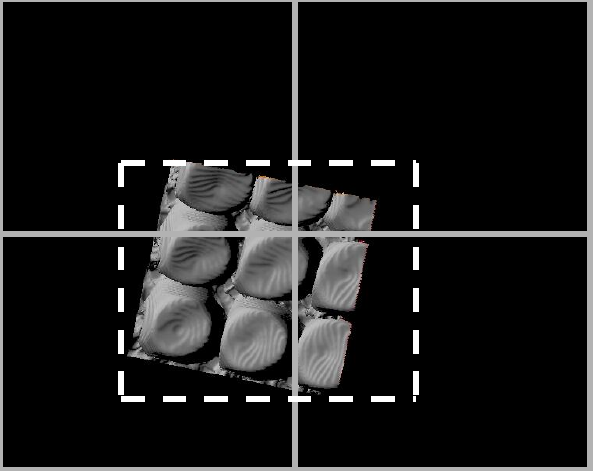
\includegraphics[width=3in]{images/FloatingViewport}
  \caption[Floating viewport.]{Even though geometry may straddle tile
    boundaries, we may be able to render it all in one pass by ``floating''
    the viewport.}
  \label{fig:FloatingViewport}
\end{figure}

Consider the geometry shown in Figure~\ref{fig:FloatingViewport} that
projects onto a screen space that fits within a single tile but is moved in
the horizontal and vertical directions so that it straddles four tiles.  If
the system limits itself to projecting onto physical tiles, the processor
must render four images even though it could generate a single
image that contains the entire geometry with the exact same pixel spacing.
Instead of rendering four tiles, \IceT can \keyterm{float} the
viewport in the global display to the space straddling the tiles.  That is,
\IceT may project the geometry to the space shown by the dotted line
in Figure~\ref{fig:FloatingViewport} and split the resulting image back
into pieces that can be displayed directly on each tile.  Hence, the system
does not need to render any polygon more than once.

When a processor's geometry fits within the floating viewport, it can cut
the rendering time dramatically.  This is most likely to happen when the
number of tiles is small compared to the number of processors and the
spatial coherency of the data is good.

The floating viewport is always enabled by default.  You can disable it by
calling \CFunc{icetDisable} with the \CEnum{ICET\_FLOATING\_VIEWPORT}
identifier.  In general, there is not much reason to turn off the floating
viewport.  The only real reason to turn off the floating viewport is to
prevent \IceT from changing the perspective matrix when in single tile
mode.  However, \IceT will change the perspective matrix anyway when
rendering with more than one tile, so any application that might render to
a tiled display should simply leave the floating viewport option on.

\index{floating~viewport|)}

\section{Active-Pixel Encoding}
\label{sec:Customizing_Compositing:Active_Pixel_Encoding}
\index{active-pixel~encoding|(}

Because each processor renders only a fraction of the total geometry, the
geometry often occupies only a fraction of the screen space in some or all
of the tiles in which it lies.  Consequently, the initial images
distributed between processors at the beginning of composition often have a
significant amount of blank space within them.  Explicitly sending this
data between processors is a waste of bandwidth.  Transferring
sparse image data rather than full image data is a well-known way to reduce
network overhead.  So far, our best method to do this has been with
active-pixel encoding.

Active-pixel encoding is a form of run-length encoding.  A traditional
run-length encoding groups pixels into contiguous groups where the color
or depth does not change.  However, in a practical 3D rendering, both
the color and depth change almost everywhere except in the background areas
where nothing is rendered.  To take advantage of this, images are grouped
into alternating run lengths of \keyterm{active pixels}, pixels that
contain geometry information, and \keyterm{inactive pixels}, pixels that
have no geometry drawn on them.  The active-pixel run length is followed by
pairs of color and depth values (or just one of the two if that is the only
data available).  The inactive pixels are not accompanied by any color or
depth information.  The depth information is assumed to be of maximum
depth, and the color values are ignored since they contain no geometry
information.

There are many other ways to encode sparse images and reduce data
redundancy.  However, we are particularly enamored with our active-pixel
encoding for this application because it exhibits all of the following
properties:

\begin{description}
\item[Fast encoding]  Image encoding requires each pixel to be visited
  exactly once.  Each visit includes a single alpha or depth comparison, a
  single addition, and at most one copy.
\item[Free decoding]  Processors typically perform a compositing as
  soon as they receive incoming data.  The compositing can be done
  directly against an image that is still encoded in sparse form.  In fact,
  the compositing can skip the comparisons for the inactive pixels.
  Thus doing compositing against encoded images is often faster than
  against unencoded images.
\item[Effective compression]  During the early stages of composition when
  the most image data must be transferred, the sparse data is commonly less
  than one fifth the size of the original data.
\item[Good worst case behavior] No image will ever grow by more than a few
  bytes of header information.  Images that have geometry drawn on every
  pixel will only have one run length.  Even images that alternate between
  active and inactive status for every pixel, and hence have a run length
  for every pixel, do not grow when encoded.  The number of bytes required
  to record two run lengths, which are stored as 16-bit integers each, is
  no more than the number of bytes saved by not recording either color or
  depth data for a single inactive pixel, which is at least 32-bits.  Thus,
  there is no penalty for recording run lengths of size one.
\end{description}

Active-pixel encoding is performed automatically during the compositing
process.  There is currently no way to turn it off.

\index{active-pixel~encoding|)}

\section{Interlaced Images}
\label{sec:Customizing_Compositing:Interlaced_Images}

\index{image!interlace|(}
\index{interlace|see{image, interlace}}

Although active pixel encoding almost always improves the performance of
compositing, it does introduce an issue of load balancing.  As images are
partitioned, some regions will have more active pixels than others.  By
balancing the active pixels assigned to regions, the parallel compositing
becomes better load balanced and performance can improve even further.

The most straightforward way of balancing active pixels is to
\keyterm{interlace} the images.  An image is interlaced by rearranging
pixels in a different order.  This reordering of pixels is designed such
that when the images are later partitioned, each partition gets pixels from
all over the images.  Consequently, regions with many active pixels are
distributed to all the partitions.

Although image interlacing can provide a significant performance increase,
it also incurs an overhead caused by shuffling pixels around.  This
overhead can potentially happen in two places during parallel compositing.
The first overhead is the shuffling of pixels before any compositing or
message transfers take place.  This overhead tends to be low because it
occurs when images are their most sparse and the work is distributed
amongst all the processes.  The second overhead is the reshuffling after
compositing completes to restore the proper order of the pixels.  This
second shuffling is substantial as it happens when images are at their most
full and the maximum amount of pixels must be copied.  Furthermore, because
pixels must be shuffled over the entire image, this reshuffling must happen
after image data is collected on a single process.  Thus, the reshuffling
happens on a single process while all others remain idle.

\index{partitioning!image}
\index{image!partitioning}
Classical implementation of image interlacing shuffle pixels in regions,
but the regions chosen are usually arbitrary (scanlines is a common region
to pick).  However, the image interlacing algorithm in \IceT chooses
regions that completely avoid the need for the second, and most time
consuming, pixel reshuffling.  The algorithm is based on the simple
observation that at the completion of many parallel compositing algorithms,
the final image is partitioned and distributed among all the processes in
contiguous pieces.  If we arrange our initial shuffling such that each of
the partitions remain a contiguous set of pixels, then we do not need the
final reshuffling at all.

\begin{figure}
  \centering
  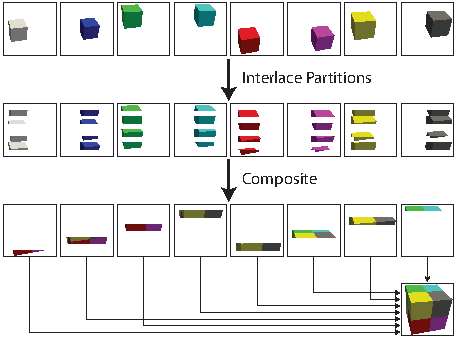
\includegraphics[width=.8\textwidth]{images/InterlaceDiagram}
  \caption{Pixel shuffling in \IceT's image interlacing.}
  \label{fig:Interlacing}
\end{figure}

\IceT's minimal-copy image interlacing is demonstrated in
Figure~\ref{fig:Interlacing}.  Rather than picking arbitrary partitions,
such as scan lines, to interlace, \IceT's interlacing uses the partitions
that the composite will create anyway.  The image with the interlaced block
is composited as normal.  Each resulting image partition is already intact,
it is only the implicit offsets that need to be adjusted.

Image interlacing is always on by default.  It can be turned off by calling
\CFunc{icetDisable} with \CEnum{ICET\_INTERLACE\_IMAGES}.  Image
interlacing is only a hint, and compositing strategies are not obligated to
follow it.  In any case, the observable behavior between interlaced and
non-interlaced images is the same except for in compositing times.  In
situations where each process renders to a small portion of an image, the
overhead for image interlacing is low but its benefits are high.  However,
in cases where every process renders geometry over the entire view
(indicative of a poor distribution of geometry), then the overhead for
image interlacing becomes higher but the benefit becomes lower.

\index{image!interlace|)}

\section{Data Replication}
\label{sec:Customizing_Compositing:Data_Replication}
\index{data~replication|(}

The primary advantage of \IceT's parallel rendering algorithms, and
sort-last rendering algorithms in general, is that they are very scalable
with respect to the size of the input geometry.  That is, there is no
overhead to adding more geometry other than the time it takes hardware to
render and there is only a logarithmic overhead for adding processors to
the job.

The down side of a sort-last approach is that the image compositing
overhead must be incurred regardless of how little geometry is being
rendered.  This overhead limits the maximum frame rate that can be achieved
by the parallel rendering.  Consequently, the parallel rendering can
potentially be slower than the serial rendering if the amount of geometry
being rendered is small.

One possible way to get higher frame rates with smaller geometries would be
to switch to a different parallel rendering mode, but doing so is
unnecessarily complicated.  Another possibility is to collect the data on
a single process and circumvent the \IceT library entirely.  This approach
is fine when using single tile mode where the image is displayed at a
single location, but is not at all straightforward when displaying to a
tiled display.

\IceT provides a better solution than either of the previous two
approaches.  If the image compositing work is dominating the rendering
time, you can set up a \keyterm{data replication group}.  To set up a data
replication group, you partition the geometry using fewer partitions than
processes, and then you share each partition with multiple processes.  The
processes that share a data partition are a replication group.  \IceT will
divide the compositing work for each replication group amongst the
processes in the group.  In essence, you are adding geometry rendering work
to remove image compositing work.

One of the most common uses for data replication groups is to simply
replicate the same geometry on all processes.  This is helpful, for
example, if your application supports lower levels of detail for
interaction.  The lower level of detail can be replicated on all
processes.  However, you could also conceivably arrange for any amount of
replication between all replicated and none replicated for a consistently
appropriate overhead as the amount of data grows.

To set up data replication groups, it is your responsibility to partition
and replicate geometry.  (\IceT knows nothing about geometry.)  You then
report what the data replication groups are with the
\CFunc{icetDataReplicationGroup} function.

\begin{Table}{3}
  \textC{void }\CFunc{icetDataReplicationGroup}\textC{(}&\textC{IceTInt}&\CArg{size}\textC{,} \\
  &\textC{const IceTInt *}&\CArg{processes}\quad\textC{);}
\end{Table}

\CFunc{icetDataReplicationGroup} simply takes an array defining the
replication group that the local process belongs to.  It is important to
ensure that all processes belonging to a group provide the same array to
\CFunc{icetDataReplicationGroup}.  As a convenience, \IceT also provides
the \CFunc{icetDataReplicationGroupColor} function that allows you to
define the data replication groups by assigning an identifier (i.e. color)
to each partition and having each process report the partition color in
which it belongs.
\begin{Table}{3}
  \textC{void }\CFunc{icetDataReplicationGroupColor}\textC{(}&\textC{IceTInt}&\CArg{color}\quad\textC{);}
\end{Table}

As an example, let us say that processes 0--3 share the same geometry, 4--7
share the same geometry, 8--11 share the same geometry, and so on.  These
replication groups could be reported with the following call (where
\textC{rank} is the local process id as stored in the \CEnum{ICET\_RANK}
state variable).
\begin{code}
icetDataReplicationGroupColor(rank/4);
\end{code}

The data replication group is stored in the
\CEnum{ICET\_DATA\_REPLICATION\_GROUP} state variable (retrievable with
\CFunc{icetGet}).  The length of the group array is stored in
\CEnum{ICET\_DATA\_REPLICATION\_GROUP\_SIZE}.  The data replication group
array is available regardless of whether you used
\CFunc{icetDataReplicationGroup} or \CFunc{icetDataReplicationGroupColor}
to define the group.  The default value is an array with one value: the
local process.

\index{data~replication|)}

\section{Compositing Network Hints}
\label{sec:Customizing_Compositing:Compositing_Network_Hints}
\index{compositing!network|(}

By its nature, image compositing requires a significant amount of
communication amongst processes in a parallel computer.  Each compositing
algorithm contained in \IceT follows a particular pattern of communication,
referred to as its \keyterm{compositing network}.  These algorithms and
their compositing networks are described in Chapter~\ref{chap:Strategies}.

Most compositing networks are fixed although a few have some possible
variability.  Any variations in the compositing networks are automatically
chosen, but it is possible to provide hints.  Because the relative
efficiency of different compositing networks is effected more by the
underlying hardware than in the application and data running it, these hints
are specified by either build options or by environment variables.

Build options are specified as \index{CMake}CMake variables.  These CMake
variables are set using the CMake program at the beginning of the build as
described in Chapter~\ref{chap:Tutorial}.  These variables are listed as
``advanced,'' so you will need to turn on advanced variables in the CMake
to see them.

For each one of these CMake build variables, \IceT also recognizes a
corresponding environment variable with the same name at run time.  If the
environment variable is defined, it will be used in place of the option set
at run time.  The environment variables are read when the \IceT context is
first created, so subsequent changes to the environment variables will have
no effect.

The following CMake and environment variable hints are available.

\begin{Description}[xxxxxxxx]
\item[\CEnum{ICET\_MAGIC\_K}] The radix-k single image strategy described
  in Chapter~\ref{chap:Strategies} starting on
  page~\pageref{sec:Strategies:Radix-k} operates by communicating within
  groups of processes of size $k$.  \IceT's implementation of radix-k
  automatically determines $k$, but does so by selecting values that are as
  close as possible to a \index{magic~k}\keyterm{magic k} value.  This
  magic k value is set with the \CEnum{ICET\_MAGIC\_K} CMake build variable
  or environment variable.
\item[\CEnum{ICET\_MAX\_IMAGE\_SPLIT}] The parallel image compositing
  algorithms in \IceT maintain load balancing by dividing images amongst
  processes to allow the processes to concurrently composite pixels in
  independent partitions of the image.  Typically, \IceT subsequently
  collects the images to the display nodes.  This collection can be one of
  the longest operations during the compositing, particularly when there
  are many processes.  It is possible to speed up the collection at the
  expense of the compositing by limiting the maximum number of times an
  image may be split.  This limit is set with the
  \CEnum{ICET\_MAX\_IMAGE\_SPLIT} CMake build variable or environment
  variable.  Be advised that this option is only a suggestion to
  compositing.  It is still possible for images to be split beyond this
  limit.  \IceT will still behave correctly either way.
\end{Description}

These values may be queried (but not set) at runtime using \CFunc{icetGet}
with a state variable identifier of the same name.

\index{compositing!network|)}

\section{Image Partition Collection}
\label{sec:Customizing_Compositing:Image_Collection}
\index{collection|(}
\index{image!collection|(}
\index{partitioning!image|(}
\index{image!partitioning|(}

Many parallel compositing algorithms, including several in \IceT, function
by partitioning images and distributing the pieces.  These algorithms,
described in more detail in Chapter~\ref{chap:Strategies}, eventually have
a composited image partitioned and distributed among most or all of the
processes involved in the operation.

For most practical purposes, such as displaying the images, the image
partitions must be collected, and by default \IceT collects each image to
its associated display process.  However, there exist some use cases where
this collection may not be necessary.  For example, if the images are only
to be written to a parallel file system, then it may be as efficient or
more efficient to collectively write partitions from multiple processes.

The collection of image data to the display process may take a significant
portion of the overall compositing time, but it is usually necessary.  When
it is not necessary, it can be disabled by calling \CFunc{icetDisable} with
\CEnum{ICET\_COLLECT\_IMAGES}.  When this option is turned off, the
strategy has the option of leaving images partitioned among processes.  Each
process containing part of a tile's image will return the entire buffer
from \CFunc{icetDrawFrame} or \CFunc{icetGLDrawFrame} in an
\CType{IceTImage} object.  However, only certain pixels will be valid.  The
state variables \CEnum{ICET\_VALID\_PIXELS\_TILE},
\CEnum{ICET\_VALID\_PIXELS\_OFFSET}, and \CEnum{ICET\_VALID\_PIXELS\_NUM}
give which tile the pixels belong to and what range of pixels are valid.

The \CEnum{ICET\_VALID\_PIXELS\_TILE} state variable gives the tile for
which the last image returned from \CFunc{icetDrawFrame} or
\CFunc{icetGLDrawFrame} contains pixels.  Each process has its own value.
If the last call to \CFunc{icetDrawFrame} or \CFunc{icetGLDrawFrame} did
not return pixels for the local process, then this state variable is set to
$-1$.

The \CEnum{ICET\_VALID\_PIXELS\_OFFSET} and
\CEnum{ICET\_VALID\_PIXELS\_NUM} give the range of valid pixels for the
last image returned from \CFunc{icetDrawFrame} or \CFunc{icetGLDrawFrame}.
Given the arrays of pixels returned with the \CFunc{icetImageGetColor} and
\CFunc{icetImageGetDepth} functions, the valid pixels start at the pixel
indexed by \CEnum{ICET\_VALID\_PIXELS\_OFFSET} and continue for
\CEnum{ICET\_VALID\_PIXELS\_NUM}.  The tile to which these pixels belong
are captured in the \CEnum{ICET\_VALID\_PIXELS\_TILE} state variable.  If
the last call to \CFunc{icetDrawFrame} or \CFunc{icetGLDrawFrame} did not
return pixels for the local process, \CEnum{ICET\_VALID\_PIXELS\_NUM} is
set to $0$.

The \CEnum{ICET\_VALID\_PIXELS\_TILE}, \CEnum{ICET\_VALID\_PIXELS\_OFFSET},
and \CEnum{ICET\_VALID\_PIXELS\_NUM} are only really useful when
\CEnum{ICET\_COLLECT\_IMAGES} is disabled.  When
\CEnum{ICET\_COLLECT\_IMAGES} is enabled, it is always the case that each
display process has the entire image (\CEnum{ICET\_VALID\_PIXELS\_TILE} set
to the tile, \CEnum{ICET\_VALID\_PIXELS\_OFFSET} set to $0$ and
\CEnum{ICET\_VALID\_PIXELS\_NUM} set to the total image size), and it is
always the case that each process not displaying a tile has no image
(\CEnum{ICET\_VALID\_PIXELS\_TILE} set to $-1$ and
\CEnum{ICET\_VALID\_PIXELS\_NUM} set to $0$).

\index{image!partitioning|)}
\index{partitioning!image|)}
\index{image!collection|)}
\index{collection|)}

\section{Timing (and Other Metrics)}
\label{sec:Customizing_Compositing:Timing}
\index{timing|(}

Whenever \CFunc{icetDrawFrame} or \CFunc{icetGLDrawFrame} is called, \IceT
measures the amount of time spent in the various tasks required for
parallel rendering.  These timings are stored in the \IceT state and can be
retrieved with \CFunc{icetGet}.  The state variables containing these
timing metrics (in seconds) are as follows.

\begin{Description}[xxxxxxxx]
\item[\CEnum{ICET\_RENDER\_TIME}] The total time spent in the drawing
  callback during the last call to \CFunc{icetDrawFrame} or
  \CFunc{icetGLDrawFrame}.
\item[\CEnum{ICET\_BUFFER\_READ\_TIME}] The total time spent copying buffer
  data and reading from \OpenGL buffers during the last call to
  \CFunc{icetDrawFrame} or \CFunc{icetGLDrawFrame}.
\item[\CEnum{ICET\_BUFFER\_WRITE\_TIME}] The total time spent writing to
  OpenGL buffers during the last call to \CFunc{icetGLDrawFrame}.  Always
  set to 0.0 after a call to \CFunc{icetDrawFrame}.
\item[\CEnum{ICET\_COMPRESS\_TIME}] The total time spent in compressing
  image data using active pixel encoding during the last call to
  \CFunc{icetDrawFrame} or \CFunc{icetGLDrawFrame}.
\item[\CEnum{ICET\_BLEND\_TIME}]/\CEnum{ICET\_COMPARE\_TIME} The total time
  spent in performing Z comparisons or color blending of images during the
  last call to \CFunc{icetDrawFrame} or \CFunc{icetGLDrawFrame}.  These two
  variables always return the same value.
\item[\CEnum{ICET\_COLLECT\_TIME}] The total time spent in collecting image
  fragments to display processes during the last call to
  \CFunc{icetDrawFrame} or \CFunc{icetGLDrawFrame}.
\item[\CEnum{ICET\_TOTAL\_DRAW\_TIME}] The total time spent in the last
  call to \CFunc{icetDrawFrame} or \CFunc{icetGLDrawFrame}.  This includes
  all the time to render, read back, compress, and composite images.
\item[\CEnum{ICET\_COMPOSITE\_TIME}] The total time spent in compositing
  during the last call to \CFunc{icetDrawFrame} or \CFunc{icetGLDrawFrame}.
  Equal to $\CEnum{ICET\_TOTAL\_DRAW\_TIME} - \CEnum{ICET\_RENDER\_TIME} -
  \CEnum{ICET\_BUFFER\_READ\_TIME} - \CEnum{ICET\_BUFFER\_WRITE\_TIME}$.
\end{Description}

In addition to timing how long rendering and compositing takes, \IceT also
keeps track of how much data is transmitted during compositing.  The state
variable \CEnum{ICET\_BYTES\_SENT} stores the total number of bytes sent by
the calling process for transferring image data during the last call to
\CFunc{icetDrawFrame}.  Obviously, each process could have a different
value for \CEnum{ICET\_BYTES\_SENT}.

\IceT also keeps track of the number of times \CFunc{icetDrawFrame} or
\CFunc{icetGLDrawFrame} has been called.  This number is stored in
\CEnum{ICET\_FRAME\_COUNT}.

\index{timing|)}
